\documentclass{beamer}
% we can make slides for widescreen display as well
%\documentclass[aspectratio=169]{beamer}

% theme: metropolis, the best modern theme there is
\usetheme{metropolis}                     

% mathematics, symbols, theorems
\usepackage{amsmath}
\usepackage{amssymb}
\usepackage{amsthm}

% let bibliography be consistent with citation style
\setbeamertemplate{bibliography item}{\insertbiblabel}

% tikz
\usepackage{tikz}

% Set up tikz for flow charts
\usetikzlibrary{shapes,arrows,positioning}

\tikzstyle{decision} = [diamond, draw, fill=red!20, text width=4.5em, text badly centered, inner sep=0pt]
\tikzstyle{block} = [rectangle, draw, fill=blue!20, text width=5em, text centered, rounded corners,
 minimum width=2cm]
\tikzstyle{line} = [draw, -latex]
\tikzstyle{doubleline} = [draw, latex-latex]
\tikzstyle{cloud} = [draw, ellipse,fill=green!20, node distance=2.5cm, minimum height=2em]
\tikzstyle{local} = [rectangle, draw, dashed, fill=yellow!10, text width=5em, text centered, rounded corners,
 minimum width=9cm, minimum height=1.4cm]
\tikzstyle{joincircle} = [circle, draw, fill=black, radius=1pt]

%%
% We can include figures with drop shadow
\usetikzlibrary{shadows,calc}
% code adapted from http://tex.stackexchange.com/a/11483/3954
% some parameters for customization
\def\shadowshift{3pt,-3pt}
\def\shadowradius{6pt}
\colorlet{innercolor}{black!60}
\colorlet{outercolor}{gray!05}
% this draws a shadow under a rectangle node
\newcommand\drawshadow[1]{
	\begin{pgfonlayer}{shadow}
		\shade[outercolor,inner color=innercolor,outer color=outercolor] ($(#1.south west)+(\shadowshift)+(\shadowradius/2,\shadowradius/2)$) circle (\shadowradius);
		\shade[outercolor,inner color=innercolor,outer color=outercolor] ($(#1.north west)+(\shadowshift)+(\shadowradius/2,-\shadowradius/2)$) circle (\shadowradius);
		\shade[outercolor,inner color=innercolor,outer color=outercolor] ($(#1.south east)+(\shadowshift)+(-\shadowradius/2,\shadowradius/2)$) circle (\shadowradius);
		\shade[outercolor,inner color=innercolor,outer color=outercolor] ($(#1.north east)+(\shadowshift)+(-\shadowradius/2,-\shadowradius/2)$) circle (\shadowradius);
		\shade[top color=innercolor,bottom color=outercolor] ($(#1.south west)+(\shadowshift)+(\shadowradius/2,-\shadowradius/2)$) rectangle ($(#1.south east)+(\shadowshift)+(-\shadowradius/2,\shadowradius/2)$);
		\shade[left color=innercolor,right color=outercolor] ($(#1.south east)+(\shadowshift)+(-\shadowradius/2,\shadowradius/2)$) rectangle ($(#1.north east)+(\shadowshift)+(\shadowradius/2,-\shadowradius/2)$);
		\shade[bottom color=innercolor,top color=outercolor] ($(#1.north west)+(\shadowshift)+(\shadowradius/2,-\shadowradius/2)$) rectangle ($(#1.north east)+(\shadowshift)+(-\shadowradius/2,\shadowradius/2)$);
		\shade[outercolor,right color=innercolor,left color=outercolor] ($(#1.south west)+(\shadowshift)+(-\shadowradius/2,\shadowradius/2)$) rectangle ($(#1.north west)+(\shadowshift)+(\shadowradius/2,-\shadowradius/2)$);
		\filldraw ($(#1.south west)+(\shadowshift)+(\shadowradius/2,\shadowradius/2)$) rectangle ($(#1.north east)+(\shadowshift)-(\shadowradius/2,\shadowradius/2)$);
	\end{pgfonlayer}
}
% create a shadow layer, so that we don't need to worry about overdrawing other things
\pgfdeclarelayer{shadow} 
\pgfsetlayers{shadow,main}

\newcommand\shadowimage[2][]{%
	\begin{tikzpicture}
	\node[anchor=south west,inner sep=0] (image) at (0,0) {\includegraphics[#1]{#2}};
	\drawshadow{image}
	\end{tikzpicture}}

%%

\title{A sample presentation in Beamer}
\date{\today}
\author{Adarsh}
\institute{Purdue University}

\begin{document}
\maketitle

% section gives a new page with only section heading (Skip if not needed)
\section{Introduction}

% one frame is one slide
\begin{frame}{Problem Statement}
	Some problem statement~\cite{tawarmalani2009allocating}
\end{frame}

% flow chart in tikz
\begin{frame}{Tikz flow chart with animation}
	\begin{center}
		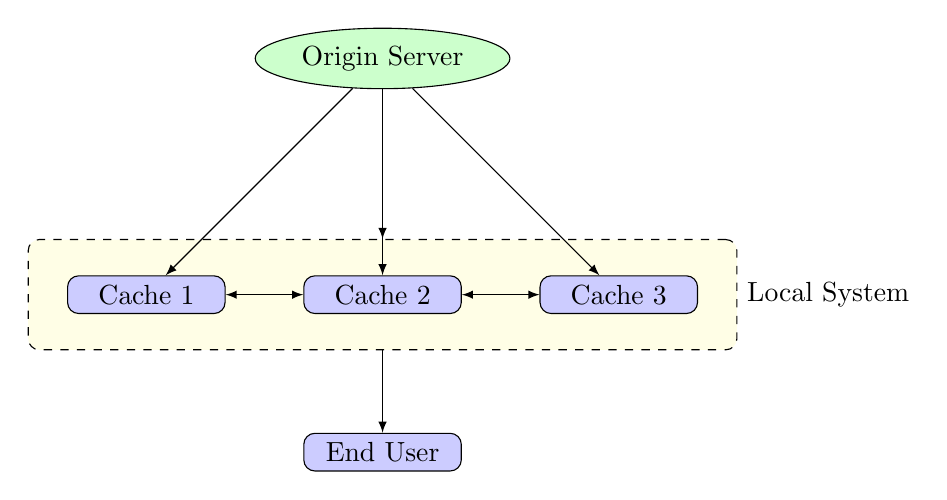
\begin{tikzpicture}[node distance=2cm]
			\node[cloud] (server) {Origin Server};
			\node [local,below of= server, label=right:{Local System}, node distance=3cm] (local) {};
			\visible<2->{\node [block,below of= server, node distance=3cm] (cache2) {Cache 2};
			\node [block,left of= cache2, node distance=3cm] (cache1) {Cache 1};
			\node [block,right of= cache2, node distance=3cm] (cache3) {Cache 3};}
			\node [block,below of= local] (user) {End User};
			\visible<2->{\path[line] (server) --          (cache1);
			\path[line] (server) --          (cache2);
			\path[line] (server) --          (cache3);
			\path[doubleline] (cache1) --          (cache2);
			\path[doubleline] (cache3) --          (cache2);
			}
			\visible<1>{\path[line] (server) --          (local);}
			\path[line] (local) --          (user);
		\end{tikzpicture}    
	\end{center}
\end{frame}

% normal line drawing in tikz
\begin{frame}{Line drawing in tikz}
	\begin{center}
		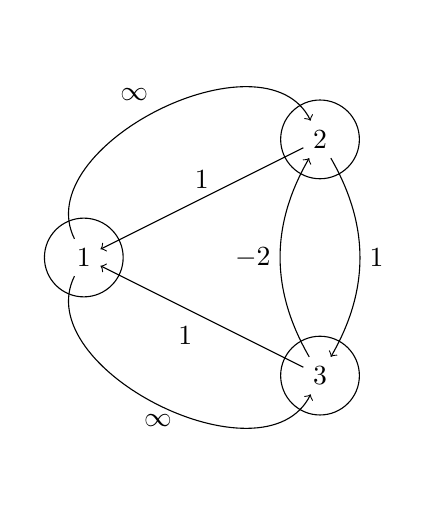
\begin{tikzpicture}
		%\draw[help lines] (-2,2) grid (4,-4);
		\draw (0,-1.5) circle (0.5cm);
		\draw (3,0) circle (0.5cm);
		\draw (3,-3) circle (0.5cm);
		\node (n1) at (0, -1.5) {1};
		\node (n2) at (3, 0) {2};
		\node (n3) at (3, -3) {3};
		\draw[bend left=90,->]  (n1) to node [auto] {$\infty$} (n2);
		\draw[ ->]  (n2) to node [above] {$1$} (n1);
		\draw[bend right=90,->]  (n1) to node [below] {$\infty$} (n3);
		\draw[->]  (n3) to node [auto] {$1$} (n1);
		\draw[bend left,->]  (n2) to node [auto] {$1$} (n3);
		\draw[bend left,->]  (n3) to node [auto] {$-2$} (n2);
		\end{tikzpicture} 
	\end{center}
\end{frame}

% figures
\begin{frame}{Including an external figure}
	\begin{figure}
		\caption{A bird}
		\centering
		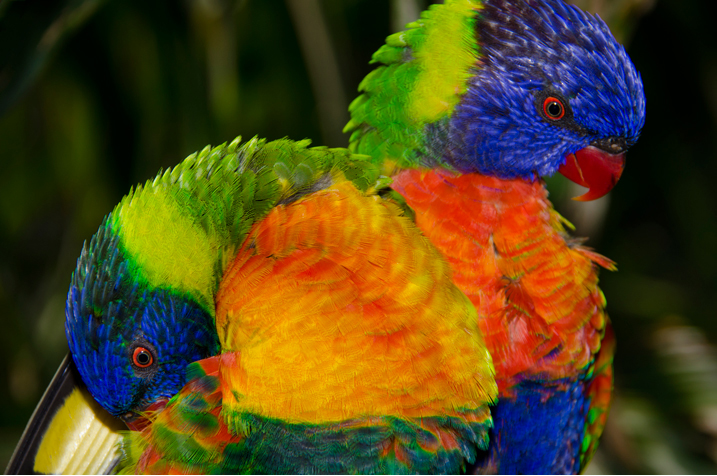
\includegraphics[scale=0.3]{../SampleImage/sample}
	\end{figure}
\end{frame}

% fancy figures
\begin{frame}{Image with drop shadow}
	\begin{figure}
		\caption{A fancy bird}
		\centering 
		\shadowimage[scale=0.3]{../SampleImage/sample}
	\end{figure}
\end{frame}

% reference
\section{Reference}
\begin{frame}{Reference}
	\bibliography{BeamerSample}
	\bibliographystyle{apalike}
\end{frame}

% thank you
\section{Thank You}
\end{document}